\section{El Teorema Fundamental del Cálculo}

\subsection{Valor promedio de una función}


 \subsection{Valor promedio de una función}
 Si una función $f$ se evalúa en $n$ puntos $\xi_{1}, \xi_{2},...,\xi_{N},$ el valor promedio de la función para estos puntos es
 $$
 \dfrac{f(\xi_{1})+f(\xi_{2})+...+f(\xi_{N})}{N}=\dfrac{1}{N}\sum_{k=1}^{N}f(\xi_{k}).
 $$



 Sin embargo, si tratamos de promediar una función en un intervalo $[a,b],$ esta definición no es útil porque habrá una infinidad\footnote{De hecho, una cantidad no numerable de puntos, por lo que ni siquiera podemos tratar de aplicar algunas técnicas para series} de puntos.


 Aun así, todavía podemos encontrar una definición, motivada por el promedio en una cantidad finita de puntos



 Escogiendo el tamaño del paso fijo para un número $N$ dado de subintervalos, tenemos que
 $$
 h=\dfrac{b-a}{N}.
 $$


 O de manera equivalente
 $$
 \dfrac{1}{N}=\dfrac{1}{b-a}h.
 $$




 De manera que
 $$
 \dfrac{1}{N}\sum_{k=1}^{N}f(\xi_{k})=\dfrac{1}{b-a}\sum_{k=1}^{N}f(\xi_{k}) \cdot h.
 $$

 Cuando $N\to \infty,$ el lado derecho se aproxima a
 $$
 \dfrac{1}{b-a} \int_{a}^{b} f(\xi)d\xi.
 $$



 \begin{definicion}
  El valor promedio de $f$ en $[a,b]$ está dado por
  $$
  \dfrac{1}{b-a} \int_{a}^{b} f(x)dx.
  $$
 \end{definicion}




 Sea $f$ una función continua en $[a,b].$ Si $x\in[a,b],$ entonces $$F(x)=\int_{a}^{x}f(\xi)d\xi$$ es una función que depende de $x$ tal que
 \[
  \label{ayr:24.2}
  D_{x}F(x)=D_{x}\left( \int_{a}^{x}f(\xi)d\xi \right)=f(x).
 \]



\subsection{Enunciado del T.F.C}


 \begin{teorema}[Teorema Fundamental del Cálculo]
  Sea $f$ una función continua en $[a,b]$ y
  $F(x)$ una antiderivada de $f(x).$ Entonces
  \[
   \label{ayr:24.3}
   \tag{TFC}
   \int_{a}^{b}f(\xi)d\xi=F(b)-F(a).
  \]

 \end{teorema}




 La ecuación \eqref{ayr:24.3} nos da una manera sencilla de calcular $$\int_{a}^{b}f(\xi)d\xi...$$ \emph{siempre y cuando podamos encontrar una antiderivada de $f(x)$, en términos de funciones elementales.}



 La expresión $F(b)-F(a)$ generalmente se abrevia como $$F(x)\mid_{a}^{b}.$$



 Calcule las siguientes fórmulas utilizando el \eqref{ayr:24.3}:
 \begin{enumerate}
  \item $$\int_{a}^{b}x dx=$$
  \item $$\int_{a}^{b}x^{2} dx=$$
  \item $$\int_{a}^{b}x^{r} dx=$$
 \end{enumerate}




 \begin{proposicion}[TFC con Cambio de Variables]
 Supongamos que en el intervalo $[a,b],$ la función $f$ es continua y la función $g$ es diferenciable.

 Entonces{\color{blue}
  $$
  \int_{a}^{b}f(g(x))g'(x)dx=
  \int_{g(a)}^{g(b)}f(u)du,
  $$}
donde {\color{green}$u=g(x).$}
 \end{proposicion}




 \begin{resuelto}
  \label{ayr:exmp:24.2}
  Evalue $$
  \int_{1}^{9}\sqrt{5x+4}dx.
  $$
 \end{resuelto}



\subsection{Ejemplos Resueltos}


 \begin{resuelto}
  Evalúe $$\int_{0}^{\pi/2} \sin^{2}(x)\cos(x)dx.$$
 \end{resuelto}




 \begin{resuelto}
  Encuentre el área de la región entre la curva dada por $f(x)=\dfrac{1}{\sqrt{4-x^{2}}},$ el eje $x,$ $x=0$ y $x=1.$

 \end{resuelto}




 \begin{figure}
 \centering
 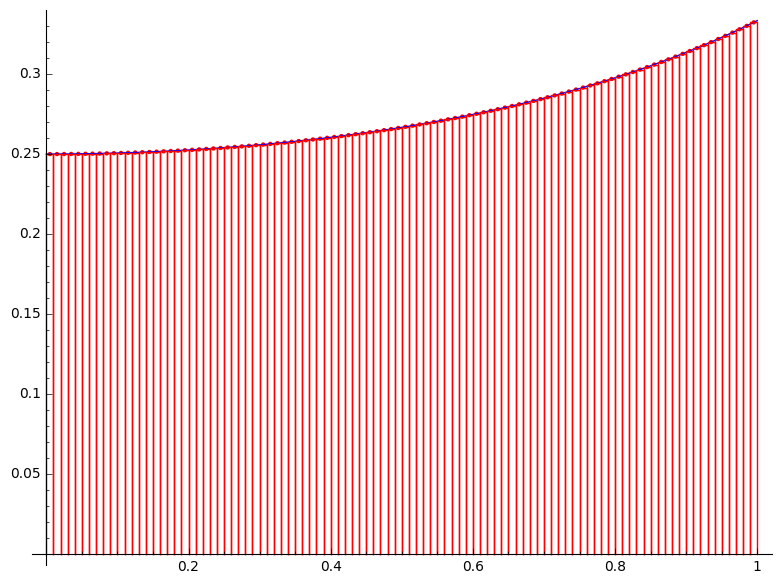
\includegraphics[height=5cm,keepaspectratio=true]{./calculo/sage0.png}
 % sage0.png: 0x0 pixel, 300dpi, 0.00x0.00 cm, bb=
 \caption{$f(x)=\dfrac{1}{\sqrt{4-x^{2}}}$}
 \label{fig:solved:24.2}
\end{figure}




 \begin{resuelto}
  Encuentre el valor promedio de $f(x)=4-x^{2}$ en $[0,2].$
 \end{resuelto}




 \begin{resuelto}
  Demuestre la fórmula \eqref{ayr:24.2}. Sugerencia: Utilice el teorema del valor medio.
 \end{resuelto}




 \begin{teorema}[Teorema del Valor Medio para Integrales]
 Sea $f$ una función continua en $[a,b].$  Entonces existe $c\in[a,b]$ tal que
 \[
  \label{ayr:24.1}
  \int_{a}^{b}f(\xi)d\xi = \left( b-a \right)f(c)
 \]
\end{teorema}



 \begin{resuelto}
  Demuestre que
  \begin{enumerate}
   \item Si $f$ es una función par, entonces
   para $a>0:$
   $$
   \int_{-a}^{a}f(x)dx=2 \int_{0}^{a}f(x)dx;
   $$
   \item Si $f$ es una función impar, entonces
   para $a>0:$
   $$
   \int_{-a}^{a}f(x)dx=0.
   $$
  \end{enumerate}

 \end{resuelto}




 \begin{resuelto}[Regla trapezoidal]
  Sea $f(x)\geq 0$ en $[a,b].$ Dividamos $[a,b]$ en $N$ subintervalos de longitud fija $h=\frac{b-a}{N},$ por medio de puntos
  $$x_{k}=a+k\cdot h, \; k=1,...,N.$$


  Muestre que $$
  \int_{a}^{b}f(\xi)d\xi \approx
  \frac{h}{2} \left( f(a)+2\sum_{k=1}^{N-1}f(\xi_{k})+f(b) \right)
  $$
 \end{resuelto}




 \begin{figure}
 \centering
 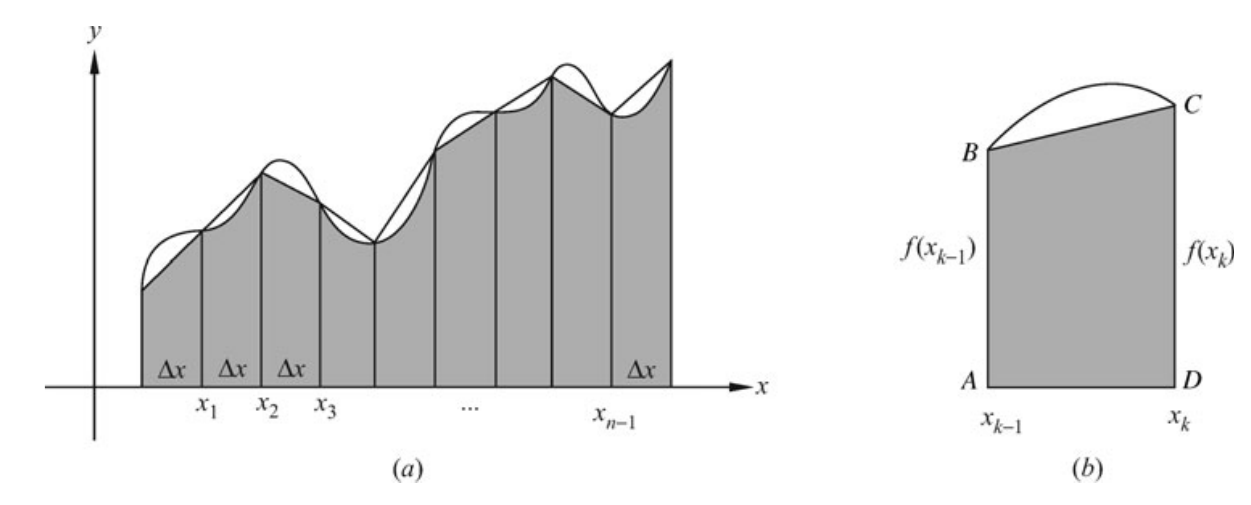
\includegraphics[width=10cm,keepaspectratio=true]{./calculo/trapezoid.png}
 % trapezoid.png: 0x0 pixel, 300dpi, 0.00x0.00 cm, bb=
 \caption{Regla trapezoidal}
 \label{fig:ayr:24.2}
\end{figure}





 \begin{resuelto}
  Use la regla trapezoidal para aproximar
  $$
  \int_{0}^{1}x^{2}dx
  $$ con $N=1.$


  Utilice el \eqref{ayr:24.3} para calcular la integral de manera exacta y compare.
 \end{resuelto}


